\documentclass[11pt]{article}

\usepackage[margin=1in]{geometry}
\usepackage[T1]{fontenc}
\usepackage[utf8]{inputenc}
\usepackage{lmodern}
\usepackage{microtype}
\usepackage{amsmath,amssymb,amsfonts}
\usepackage{graphicx}
\usepackage{booktabs}
\usepackage{tabularx}
\usepackage{multirow}
\usepackage{enumitem}
\usepackage{hyperref}
\usepackage{xcolor}
\usepackage{listings}
\usepackage{caption}
\usepackage{subcaption}

\hypersetup{
  colorlinks=true,
  linkcolor=blue!60!black,
  citecolor=blue!60!black,
  urlcolor=blue!60!black,
}

\newcommand{\cmark}{$\checkmark$}
\newcommand{\xmark}{$\times$}
\newcommand{\arxivcomment}[1]{\textcolor{gray}{\small #1}}

\DeclareMathOperator{\relu}{relu}

\lstset{
  basicstyle=\ttfamily\small,
  breaklines=true,
  frame=single,
  framesep=4pt,
  backgroundcolor=\color{gray!8},
  showstringspaces=false,
  commentstyle=\color{gray!60!black}\itshape,
  morecomment=[l]{\#},
}

\title{%
  \textbf{PsiLogic: Chaos-Aware Active Cancellation for Adam\\
  with a Fair Cross-Domain Benchmark}%
}
\author{%
  \textbf{Ali Sultonov}\\
  Independent Researcher\\
  \texttt{troxtergrif@gmail.com}\\
  \url{https://github.com/Troxter222/psilogic}%
}
\date{}

\begin{document}
\maketitle

\begin{abstract}
Adam and AdamW apply one update rule whether early gradients are noisy or the run
has already settled. We introduce \textbf{PsiLogic} ($\Psi$Logic), which adds a
dynamic Active Cancellation term to Adam. The term is gated by a dual exponential
moving average (EMA) of scale-normalized gradient norms. This chaos detector
increases damping when those statistics are unstable and fades to zero as training
settles, so early steps are damped without a separate warmup schedule.

We compare PsiLogic with Adam, AdamW, and Lion under \textbf{FairBench}. Each
optimizer gets its own learning-rate sweep, runs that share a seed start from the
same initialization, and differences are Welch $t$-tests. On an NVIDIA H100 80GB
reference run (4 arenas, 3 seeds, 2000 steps, bf16 AMP), PsiLogic has the best
validation metric on NLP perplexity and ViT accuracy, beats Adam on ResNet (the
gap vs.\ AdamW is not significant), and ties Adam/AdamW on diffusion.
NLP perplexity is $7.79 \pm 0.18$ vs.\ $8.17 \pm 0.08$ (AdamW, $p = 0.049$);
ViT top-1 is $0.244 \pm 0.006$ vs.\ $0.223 \pm 0.002$ (AdamW, $p = 0.015$);
ResNet top-1 is $0.222 \pm 0.001$ vs.\ Adam $0.172 \pm 0.004$ ($p = 0.001$) and
AdamW $0.219 \pm 0.005$ ($p = 0.44$, n.s.); diffusion MSE is
$0.02009 \pm 0.00045$ vs.\ $0.01987 \pm 0.00006$ ($p = 0.49$, n.s.). Peak GPU
memory is similar across optimizers. On the June 2026 H100 run, before Triton
fusion, wall time was 1.2--1.8$\times$ AdamW (Section~\ref{sec:limitations}).
Package v0.5+ includes an optional fused CUDA backend with the same update. A
fused FairBench re-run is not in this preprint.

The PyTorch implementation, the FairBench harness, and the raw CSV outputs are public.

\medskip
\noindent\textbf{Keywords:} optimization, Adam, adaptive learning rate, deep learning, reproducibility
\end{abstract}

\section{Introduction}

The optimizer changes how fast a model converges, how stable the run is, and often
the final metric. Adam~\cite{kingma2015adam} and AdamW~\cite{loshchilov2019adamw} are
what most training code uses. Their update does not depend on whether the current
gradient statistics look unstable or already quiet. At initialization gradients are
large and noisy; near convergence they are small. Adam applies the same kind of step
in both cases.

\textbf{PsiLogic} adds a chaos-conditioned damping term to the Adam update. The term
is largest when a dual EMA of normalized gradient norms indicates a spike, and it
goes to zero on its own as training settles. It is a drop-in for
\texttt{torch.optim.Adam}, with optional task presets
(\texttt{PsiLogicNLP}, \texttt{PsiLogicGPT}, \texttt{PsiLogicViT}).

\paragraph{Contributions.}
\begin{enumerate}[leftmargin=*, itemsep=2pt]
  \item Chaos-gated Active Cancellation on Adam, with unified decay and optional
    gradient centralization (GC) and adaptive gradient clipping (AGC).
  \item FairBench: a per-optimizer LR sweep, identical weights per seed, four task
    arenas, and Welch $t$-tests.
  \item A reference H100 run. CSVs and learning curves are in
    \texttt{benchmark/results/full/}. Ties and non-significant comparisons are in
    the tables, not only the wins.
\end{enumerate}

Diffusion ties Adam/AdamW. ResNet vs.\ AdamW is not significant at three seeds.
Step time on the June 2026 run is slower than AdamW
(Section~\ref{sec:limitations}).

\section{Related Work}
\label{sec:related}

\paragraph{Adaptive first-order methods.}
Adam~\cite{kingma2015adam} keeps bias-corrected first- and second-moment estimates and
uses them as per-parameter rates. AdamW~\cite{loshchilov2019adamw} splits weight decay
out of the gradient step. That is the usual setup for Transformers.
AdaFactor~\cite{shazeer2018adafactor} cuts memory with factored second-moment estimates.
Lion~\cite{chen2023lion} uses a sign update and coupled weight decay. It uses less
memory, and it often needs its own LR.

\paragraph{Large-batch and layer-wise scaling.}
LARS~\cite{you2017lars} and LAMB~\cite{you2019lamb} rescale updates by the ratio of
parameter norm to gradient norm, which is what makes very large minibatches trainable.
They fix scale mismatch across layers. They do not turn damping on and off from online
gradient volatility.

\paragraph{Second-order and curvature-aware methods.}
Shampoo~\cite{gupta2018shampoo} and Sophia~\cite{liu2023sophia} use richer curvature
or Hessian information. That can converge faster, and it costs more per step. PsiLogic
stays in the first-order Adam family and adds only scalar chaos statistics, shared
across parameters.

\paragraph{Automatic learning-rate and warmup.}
Manual LR warmup~\cite{goyal2017large} is standard for large-batch SGD and Transformers.
Hypergradient descent~\cite{baydin2017hypergrad} differentiates through the optimizer to adapt
the LR online. Recent \emph{parameter-free} methods such as D-Adaptation~\cite{defazio2023dadapt}
and Prodigy~\cite{mishchenko2023prodigy} estimate a suitable global step size from observed
gradients. PsiLogic's version of the early-phase effect is chaos-driven implicit warmup:
damping rises when gradient statistics are unstable and fades without an external schedule.

\paragraph{Stability mechanisms.}
Gradient centralization~\cite{yong2020gc} and adaptive gradient
clipping~\cite{brock2021nfn} are the usual extra stabilizers. PsiLogic can use both.
Active cancellation is a different knob: it shrinks weights when chaos is high, rather
than only rescaling or clipping gradients.

\paragraph{Optimizer evaluation.}
A shared learning rate is a common way one optimizer looks better than it is.
FairBench gives each optimizer its own LR search.

\section{Method}

\subsection{Notation and Per-Group Hyperparameters}

PsiLogic works on parameter groups indexed by $k$. Each group has a learning rate $\eta$,
AdamW weight decay $\lambda$, chaos gain $\gamma$, and a chaos amplification factor
$P_k \ge 0$ (called \texttt{p\_ext} in the code, default $1.0$). Presets use $P_k$ to put
more cancellation on some groups (embeddings, for example) and less on others, without
changing the global chaos signal. $\mathbf{g}_t = \nabla_\theta \mathcal{L}$ is the gradient
at step $t$. $w_t \in [0,1]$ is the chaos warmup weight (Section~\ref{sec:warmup}).

\subsection{Update Rule}

Each step applies unified multiplicative decay, then the bias-corrected Adam step.
The composed update is
\begin{equation}
  \theta_{t+1}
  = \theta_t \cdot (1 - \delta_t)
    - \eta \cdot \frac{\hat{m}_t}{\sqrt{\hat{v}_t} + \varepsilon}\,,
  \label{eq:update}
\end{equation}
where $\hat{m}_t$ and $\hat{v}_t$ are the usual bias-corrected Adam moments (the hat means
the same thing in Listing~\ref{lst:psilogic}) and $\delta_t$ is the unified-decay coefficient
(Section~\ref{sec:decay}). Listing~\ref{lst:psilogic} is that sequence in code order.

\subsection{Chaos Detector}

Let $\mathrm{gn}_t = \|\mathbf{g}_t\|_2 / \sqrt{\mathrm{numel}}$ be the scale-normalized gradient norm. We maintain:
\begin{align}
\mathrm{fast}_t &= 0.90 \cdot \mathrm{fast}_{t-1} + 0.10 \cdot \mathrm{gn}_t \\
\mathrm{slow}_t &= 0.99 \cdot \mathrm{slow}_{t-1} + 0.01 \cdot \mathrm{gn}_t \\
\mathrm{ratio}_t &= \mathrm{fast}_t / (\mathrm{slow}_t + \varepsilon) \\
\mathrm{chaos}_t &= \tanh(\mathrm{slow}_t) \cdot \bigl(1 + 0.5 \cdot \tanh(\relu(\mathrm{ratio}_t - 1))\bigr)
\end{align}
The fast and slow EMAs have effective horizons of about $10$ and $100$ steps.
In adaptive mode (the default), cancellation turns on when $\mathrm{fast}_t > \tau_{\mathrm{scale}} \cdot \mathrm{slow}_t$
($\tau_{\mathrm{scale}} = 2.0$). That is a relative spike, not a threshold on the raw gradient.
As $\mathrm{slow}_t \to 0$ at convergence, $\mathrm{chaos}_t \to 0$, and PsiLogic reduces toward
AdamW-like behavior.

\subsection{Unified Decay}
\label{sec:decay}

If weight decay and active cancellation are applied as two multiplications,
$\theta(1-\eta\lambda)$ then $\theta(1-c_t)$, the product is
$(1-\eta\lambda)(1-c_t)$, which is $1 - \eta\lambda - c_t$ only to first order.
At large early-step rates the cross term $-\eta\lambda c_t$ over-damps the weights.
PsiLogic uses one coefficient per step instead.

Define the chaos warmup weight $w_t \in [0,1]$ (ramps from 0 during an initial warmup window;
Section~\ref{sec:warmup}) and the per-group spike mask $s_t \in \{0,1\}$ from the chaos gate.
The raw cancellation fraction before clamping is
\begin{equation}
  \tilde{c}_t = s_t \cdot \mathrm{chaos}_t \cdot \eta \cdot \gamma \cdot P_k.
  \label{eq:raw-cancel}
\end{equation}
We clamp and add weight decay:
\begin{equation}
  \delta_t = \eta \lambda + w_t \cdot \min\!\bigl(\tilde{c}_t,\; c_{\max}\bigr),
  \qquad c_{\max} = \texttt{max\_cancel}
  \label{eq:delta}
\end{equation}
which is the $\delta_t$ used in Eq.~\eqref{eq:update}. $\eta\lambda$ is the AdamW decay;
$w_t \cdot \min(\tilde{c}_t, c_{\max})$ is chaos-gated cancellation scaled by $P_k$;
$c_{\max}$ (default 0.05) caps per-step shrinkage while initialization is still volatile.
Optional cosine schedules on $\gamma$ are supported via \texttt{gamma\_T\_max}.

\paragraph{Optional quantum decay.}
Let $q_0 \ge 0$ denote the \texttt{quantum\_decay} hyperparameter (default $q_0 = 0$ disables the feature).
When $q_0 > 0$, an effective rate $q_t$ is cosine-scheduled over training alongside $\gamma$
via \texttt{gamma\_T\_max} (the same schedule helper used for $\gamma$).
After computing $\delta_t$ but before the Adam subtraction in Listing~\ref{lst:psilogic}, each coordinate
is multiplied by
\begin{equation}
  \rho_{t,i} = 1 - \eta\, q_t\, w_t\, (1 - s_t)\, \tanh\!\bigl(|g_{t,i}|\bigr),
  \label{eq:quantum-rho}
\end{equation}
but only when $s_t = 0$, so auxiliary gradient-dependent regularization does not stack with
active cancellation on spike steps. FairBench presets use $q_0 = 0$ unless noted.

\subsection{Chaos Warmup}
\label{sec:warmup}

For \texttt{chaos\_warmup}$=-1$, the warmup horizon auto-scales as
$\max(500,\, T/20)$ over $T$ training steps. While $t \le t_{\mathrm{warm}}$, $w_t=0$; then
$w_t$ ramps linearly to $1$ over $t_{\mathrm{warm}}/4$ steps. This prevents the chaos term from firing on raw from-scratch gradient noise.

\subsection{Algorithm}

\begin{lstlisting}[caption={PsiLogic (simplified; matches Eqs.~\ref{eq:delta}, \ref{eq:update}).},
                    label={lst:psilogic}]
for t = 1 ... T:
    grad <- nabla L(theta); optionally apply AGC and gradient centralization
    update Adam moments m, v; update fast_t, slow_t from ||grad||_2
    s_t <- spike mask from chaos gate
    c_t <- min(s_t * chaos_t * eta * gamma * P_k, max_cancel)
    delta <- eta*lambda + w_t*c_t
    theta <- theta * (1 - delta)          # unified decay
    # optional quantum decay when q_0 > 0:
    theta <- theta * (1 - eta*q_t*w_t*(1-s_t)*tanh(abs(grad)))
    theta <- theta - eta * m_hat / (sqrt(v_hat) + eps)   # Adam step
\end{lstlisting}
Full implementation: \url{https://github.com/Troxter222/psilogic} (\texttt{psilogic/optimizer.py}).

\subsection{Comparison with Baselines}

\begin{table}[t]
  \centering
  \caption{Feature comparison of optimizers.}
  \label{tab:features}
  \small
  \begin{tabular}{lcccc}
    \toprule
    Property & Adam & AdamW & Lion & \textbf{PsiLogic} \\
    \midrule
    Per-parameter adaptive rates & \cmark & \cmark & \xmark & \cmark \\
    Unified decay (with chaos) & \xmark & \xmark & \xmark & \cmark \\
    Chaos-aware damping & \xmark & \xmark & \xmark & \cmark \\
    Implicit early-phase damping & \xmark & \xmark & \xmark & \cmark \\
    Batched \texttt{foreach} CUDA kernels & partial & \cmark & \xmark & \cmark \\
    \bottomrule
  \end{tabular}
\end{table}

\section{FairBench Evaluation}

\subsection{Protocol and Arenas}

All headline numbers are from one run on an NVIDIA H100 80GB HBM3
(PyTorch 2.4.1+cu124, CUDA 12.4). The config is
\texttt{benchmark/results/full/config.json}. FairBench has two stages:
(1)~a per-optimizer LR sweep over 7 log-spaced rates from $10^{-5}$ to $10^{-2}$
(500 steps each); (2)~evaluation at the selected LR for 2000 steps, seeds $\{0,1,2\}$,
identical initialization. Shared settings: batch 64, bf16 AMP, grad clip 1.0, cosine LR,
100-step warmup. Four arenas: NLP (Small GPT / TinyStories), ViT-Tiny on CIFAR-100,
ResNet-18 on Tiny ImageNet, and DDPM on CelebA $64^2$.
The full protocol and arena tables are in Appendix~\ref{app:protocol}.
PsiLogic uses fixed per-arena presets. Only the learning rate is tuned, same as the baselines.

\subsection{Main Results}

\begin{table}[t]
  \centering
  \caption{Main FairBench results (mean $\pm$ std over 3 seeds). Best per row in bold.}
  \label{tab:main}
  \small
  \setlength{\tabcolsep}{4pt}
  \begin{tabular}{llcccc}
    \toprule
    Arena & Metric & Adam & AdamW & Lion & \textbf{PsiLogic} \\
    \midrule
    NLP & Perplexity $\downarrow$ & $13.66 \pm 0.22$ & $8.17 \pm 0.08$ & $21.04 \pm 1.41$ & $\mathbf{7.79 \pm 0.18}$ \\
    NLP & Val loss $\downarrow$ & $2.614 \pm 0.016$ & $2.101 \pm 0.010$ & $3.045 \pm 0.068$ & $\mathbf{2.053 \pm 0.023}$ \\
    ViT & Val acc $\uparrow$ & $0.079 \pm 0.003$ & $0.223 \pm 0.002$ & $0.213 \pm 0.002$ & $\mathbf{0.244 \pm 0.006}$ \\
    ResNet & Val acc $\uparrow$ & $0.172 \pm 0.004$ & $0.219 \pm 0.005$ & $0.205 \pm 0.007$ & $\mathbf{0.222 \pm 0.001}$ \\
    Diffusion & Val MSE $\downarrow$ & $0.01987 \pm 0.00006$ & $0.01987 \pm 0.00006$ & $0.02175 \pm 0.00025$ & $0.02009 \pm 0.00045$ \\
    \bottomrule
  \end{tabular}
\end{table}

\noindent\textbf{Selected LRs.} NLP: all $3.16 \times 10^{-4}$. ViT: Adam $3.16 \times 10^{-5}$,
AdamW/PsiLogic $3.16 \times 10^{-4}$, Lion $10^{-4}$. ResNet: Adam/Lion $10^{-4}$,
AdamW/PsiLogic $3.16 \times 10^{-4}$. Diffusion: Adam/AdamW/PsiLogic $10^{-3}$, Lion $10^{-4}$.
Welch $t$-tests, compute costs, and per-seed numbers are in
Appendix~\ref{app:sig}--\ref{app:seeds}.

\subsection{Learning Curves and Overhead}

\begin{figure}[t]
  \centering
  \begin{subfigure}[b]{0.48\linewidth}
    \centering
    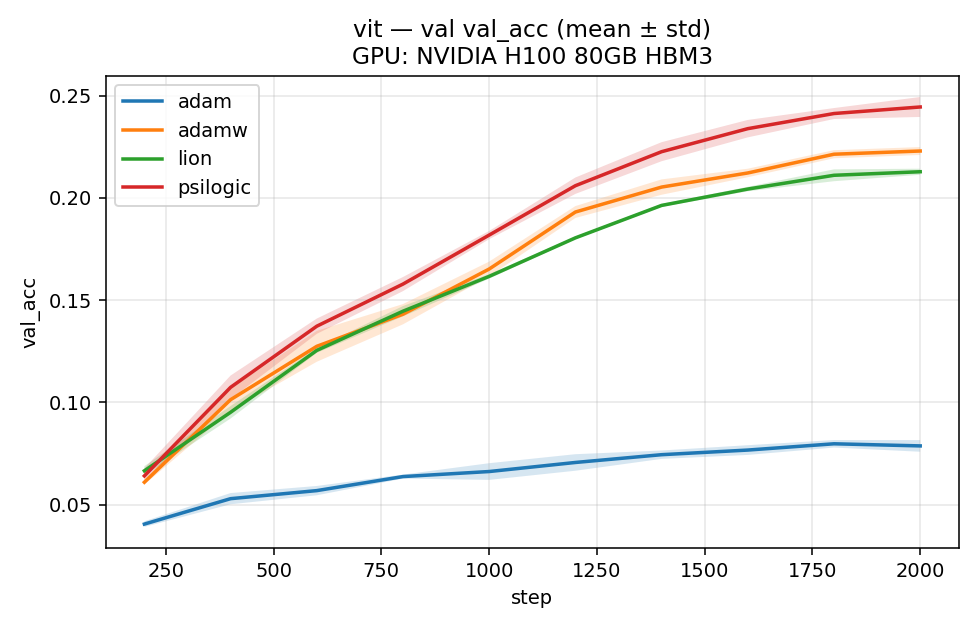
\includegraphics[width=\linewidth]{figures/vit_val_val_acc.png}
    \caption{ViT val.\ accuracy.}
    \label{fig:vit}
  \end{subfigure}\hfill
  \begin{subfigure}[b]{0.48\linewidth}
    \centering
    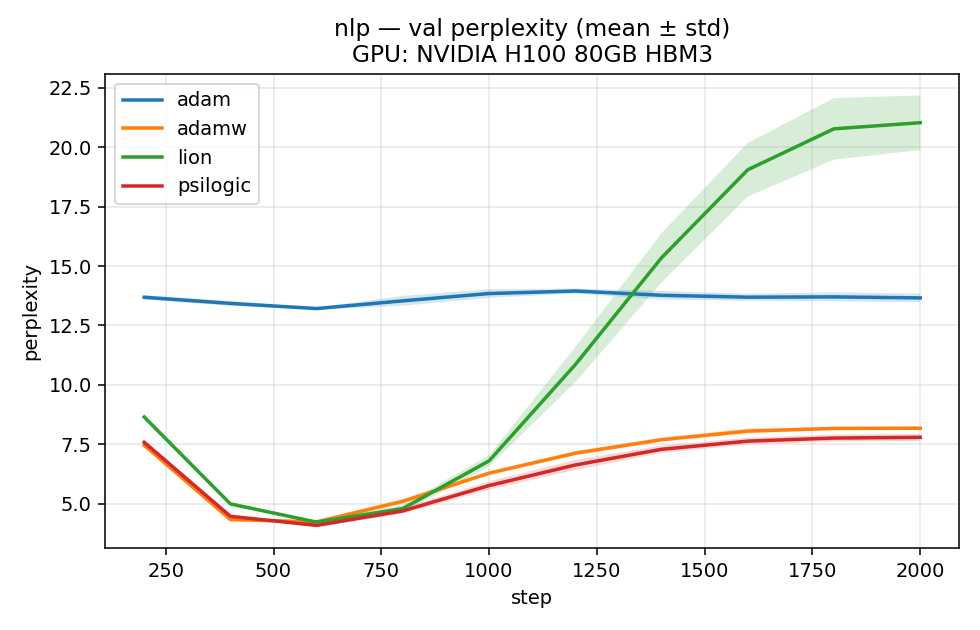
\includegraphics[width=\linewidth]{figures/nlp_val_perplexity.png}
    \caption{NLP perplexity.}
    \label{fig:nlp}
  \end{subfigure}\\[0.6em]
  \begin{subfigure}[b]{0.48\linewidth}
    \centering
    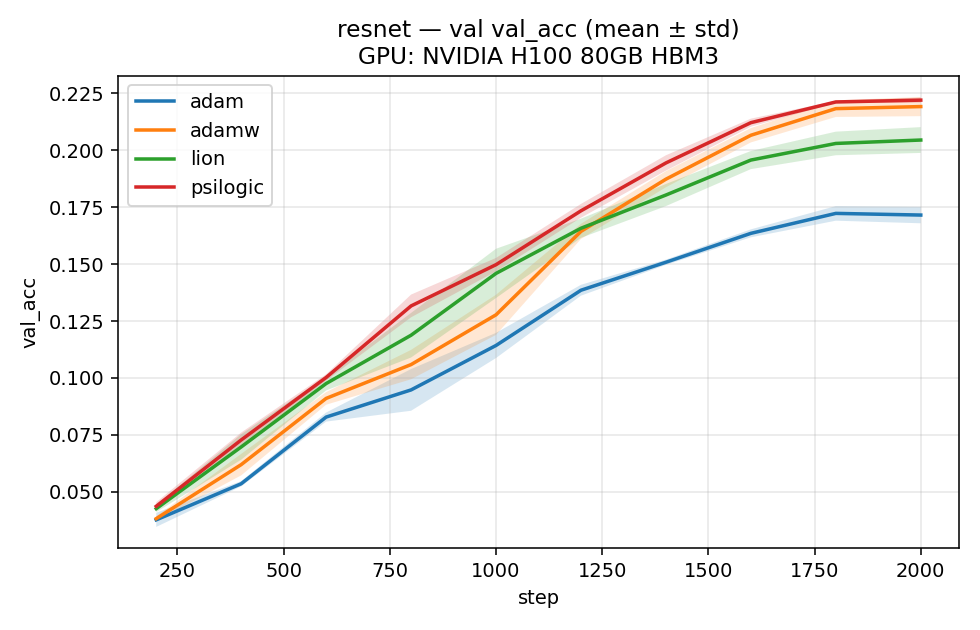
\includegraphics[width=\linewidth]{figures/resnet_val_val_acc.png}
    \caption{ResNet top-1 acc.}
    \label{fig:resnet}
  \end{subfigure}\hfill
  \begin{subfigure}[b]{0.48\linewidth}
    \centering
    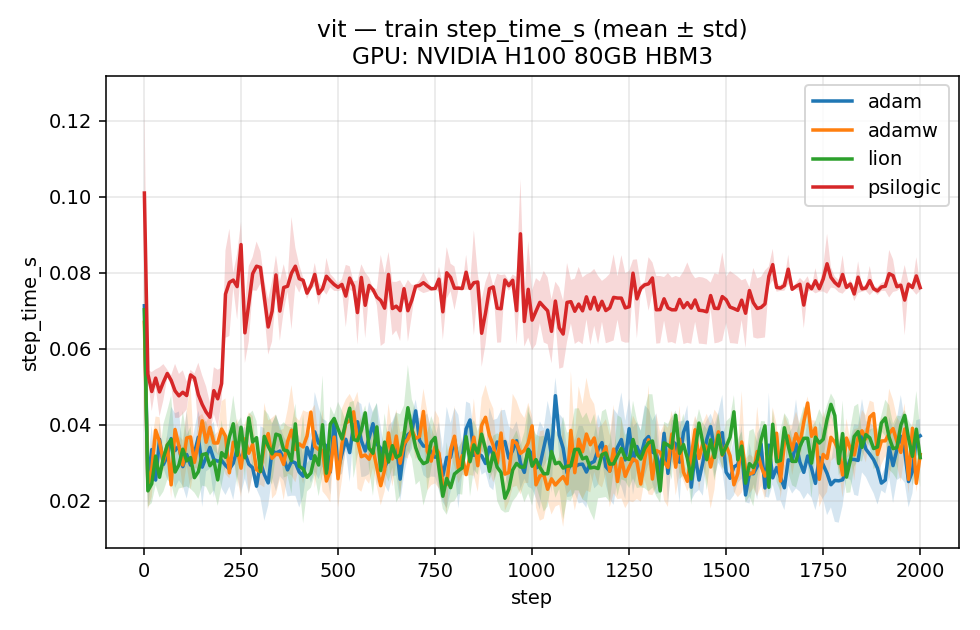
\includegraphics[width=\linewidth]{figures/vit_train_step_time_s.png}
    \caption{ViT step time.}
    \label{fig:overhead}
  \end{subfigure}
  \caption{FairBench learning curves (mean $\pm$ std) and ViT per-step wall-time overhead on H100.}
  \label{fig:curves}
\end{figure}

PsiLogic has the best NLP perplexity and ViT accuracy in Table~\ref{tab:main}.
It beats Adam on ResNet. The edge over AdamW there ($0.222$ vs.\ $0.219$) is not
significant at three seeds ($p=0.44$). Diffusion ties Adam/AdamW.
Against Adam, the NLP, ViT, and ResNet gains are significant
(Appendix~\ref{app:sig}). Against AdamW, ViT and NLP perplexity are significant.
Step-time overhead reaches 1.79$\times$ on ViT (Figure~\ref{fig:curves}, panel~d).
The chaos detector itself is a few scalars; the extra time on this run is in the
step implementation (Section~\ref{sec:limitations}).

\section{Ablations and Component Analysis}

Prior ablations on a synthetic MLP (v0.3.x) found that gradient centralization and
adaptive gradient clipping each help stability when combined with the chaos term.
A mirror ablation set AdamW's weight decay to PsiLogic's cancellation magnitude at
each step. That did not reproduce PsiLogic's per-parameter behavior, so the chaos
signal is not the same thing as one global weight-decay schedule.

Those runs predate FairBench. Component tests are in \texttt{tests/}. FairBench-scale
ablations of $\gamma$, \texttt{max\_cancel}, and \texttt{chaos\_warmup} are not in
this preprint.

\section{Discussion}

\paragraph{Why the damping helps.}
The ViT gap vs.\ Adam ($0.244$ vs.\ $0.079$) is large and shows up early. The chaos
term is a plausible reason: it cuts the step when gradient statistics are still
swinging. After a per-optimizer LR sweep, NLP perplexity still favors PsiLogic
over AdamW.

\paragraph{Implicit warmup.}
The cancellation term also shrinks the effective step during those swings. That is
similar to LR warmup, except the amount comes from the gradient statistics instead
of a step counter. Related to the hypergradient and parameter-free LR methods in
Section~\ref{sec:related}, but a different mechanism.

\paragraph{Seed spread.}
On ResNet, PsiLogic has the smallest cross-seed standard deviation of the four
($\pm 0.001$ on accuracy). Three seeds is a thin estimate of that.

\paragraph{Limitations.}
\label{sec:limitations}
\begin{enumerate}[leftmargin=*, itemsep=2pt]
  \item Three seeds. ResNet vs.\ AdamW and diffusion vs.\ AdamW are not significant.
  \item 2000 steps per arena. Not ImageNet-scale, and not LLM-scale.
  \item Step time up to 1.79$\times$ AdamW on ViT (June 2026 H100, before fusion).
    The chaos detector is a few scalars. The extra time on that run is in the step
    implementation. v0.5+ adds an optional Triton fused CUDA step
    (\texttt{psilogic[cuda]}, \texttt{use\_fused\_cuda=True}) with the same update,
    aimed at $\leq 1.25\times$ AdamW step time on Ampere+. A fused FairBench H100
    re-run is not in this preprint.
  \item No quality win on diffusion over Adam/AdamW at this budget.
  \item No convergence proof. The stability claims are empirical.
  \item It has not been replicated outside this repository.
  \item From v0.6 the bare constructor disables AGC and gradient centralization.
    Task presets and FairBench arena configs may still enable them. Record the
    preset if you compare against this paper.
\end{enumerate}

\section{Reproducibility Statement}

\begin{lstlisting}
git clone https://github.com/Troxter222/psilogic
cd psilogic && pip install -e ".[benchmark]" && pip install -r benchmark/requirements.txt
cd benchmark
python -m fairbench.download --data-root ./data
python -m fairbench --data-root ./data --output-dir results/full
\end{lstlisting}
Reference outputs: \texttt{benchmark/results/full/\{aggregate,summary,significance\}.csv}\\
Software DOI: \texttt{10.5281/zenodo.18739857} \quad PyPI: \texttt{pip install psilogic}

\section{Conclusion}

PsiLogic adds a chaos-gated Active Cancellation term to Adam. The term is large
while gradient statistics are unstable and goes to zero at convergence. On the H100
FairBench run it wins NLP perplexity and ViT accuracy, beats Adam and ties AdamW on
ResNet, and ties on diffusion. Wall time on that run was 1.2--1.8$\times$ AdamW,
before fusion. Still open: a fused re-run, more seeds, longer training, and a
replication that is not this repo.

\bibliographystyle{plain}
\begin{thebibliography}{99}
\bibitem{baydin2017hypergrad}
A.~G. Baydin, R.~Cornish, M.~Rubinstein, and D.~M. Wood.
Online learning rate adaptation with hypergradient descent. \emph{ICLR}, 2018.

\bibitem{brock2021nfn}
A.~Brock, et al.
High-performance large-scale image recognition without normalization. \emph{ICML}, 2021.

\bibitem{chen2023lion}
X.~Chen, C.~Liang, D.~Huang, E.~Real, K.~Wang, Y.~Liu, et al.
Symbolic discovery of optimization algorithms. \emph{NeurIPS}, 2023.

\bibitem{defazio2023dadapt}
M.~Defazio and K.~Mishchenko.
Learning-rate-free learning by D-Adaptation. \emph{ICML}, 2023.

\bibitem{goyal2017large}
P.~Goyal, et al.
Accurate, large minibatch SGD. \emph{arXiv preprint} \href{https://arxiv.org/abs/1706.02677}{arXiv:1706.02677}, 2017.

\bibitem{gupta2018shampoo}
V.~Gupta, T.~Koren, and Y.~Singer.
Shampoo: Preconditioned stochastic tensor optimization. \emph{ICML}, 2018.

\bibitem{kingma2015adam}
D.~P. Kingma and J.~Ba.
Adam: A method for stochastic optimization. \emph{ICLR}, 2015.

\bibitem{liu2023sophia}
H.~Liu, Z.~Shen, Y.~Li, S.~Lin, K.~Wang, and L.~Ma.
Sophia: A scalable stochastic second-order optimizer. \emph{ICLR}, 2024.

\bibitem{loshchilov2019adamw}
I.~Loshchilov and F.~Hutter.
Decoupled weight decay regularization. \emph{ICLR}, 2019.

\bibitem{mishchenko2023prodigy}
K.~Mishchenko and M.~Defazio.
Prodigy: An expeditiously adaptive parameter-free learner. \emph{arXiv preprint} \href{https://arxiv.org/abs/2306.06169}{arXiv:2306.06169}, 2023.

\bibitem{shazeer2018adafactor}
N.~Shazeer and M.~Stern.
Adafactor: Adaptive learning rates with sublinear memory cost. \emph{ICML}, 2018.

\bibitem{yong2020gc}
H.~Yong, J.~Huang, X.~Hua, and L.~Zhang.
Gradient centralization. \emph{ECCV}, 2020.

\bibitem{you2017lars}
Y.~You, I.~Gitman, and B.~Ginsburg.
Large batch training of convolutional networks with layer-wise adaptive rate scaling. \emph{arXiv preprint} \href{https://arxiv.org/abs/1708.03888}{arXiv:1708.03888}, 2017.

\bibitem{you2019lamb}
Y.~You, J.~Li, S.~Reddi, J.~Hseu, S.~Kumar, S.~Bhojanapalli, X.~Song, J.~Demmel, and C.-J.~Hsieh.
Large batch optimization for deep learning: Training BERT in 76 minutes. \emph{ICLR}, 2020.
\end{thebibliography}

\appendix

\section{FairBench Protocol and Arenas}
\label{app:protocol}

\begin{table}[h]
  \centering
  \caption{FairBench protocol stages.}
  \label{tab:protocol}
  \small
  \begin{tabularx}{\linewidth}{lX}
    \toprule
    Stage & Description \\
    \midrule
    \textbf{Stage 1, LR sweep} & 7 log-spaced LRs from $10^{-5}$ to $10^{-2}$; 500 steps each; best val metric wins \\
    \textbf{Stage 2, evaluation} & Selected LR; 2000 steps; seeds $\{0,1,2\}$; identical init per seed \\
    \textbf{Shared} & batch=64, bf16 AMP, grad\_clip=1.0, cosine LR, 100-step warmup \\
    \textbf{Statistics} & Mean $\pm$ std; Welch $t$-test (PsiLogic vs.\ each baseline) \\
    \bottomrule
  \end{tabularx}
\end{table}

\begin{table}[h]
  \centering
  \caption{FairBench arenas.}
  \label{tab:arenas}
  \small
  \begin{tabular}{llll}
    \toprule
    Arena & Model & Dataset & Metric \\
    \midrule
    NLP & Small GPT & TinyStories & Perplexity $\downarrow$, val loss $\downarrow$ \\
    ViT & ViT-Tiny patch16 224 & CIFAR-100 @ $224^2$ & Top-1 acc $\uparrow$ \\
    ResNet & ResNet-18 & Tiny ImageNet 200 & Top-1 acc $\uparrow$ \\
    Diffusion & DDPM + UNet & CelebA @ $64^2$ & Val MSE $\downarrow$ \\
    \bottomrule
  \end{tabular}
\end{table}

\section{Statistical Significance}
\label{app:sig}

\begin{table}[h]
  \centering
  \caption{Welch $t$-test: PsiLogic vs.\ baseline. $^{*}p<0.05$, $^{**}p<0.01$, $^{***}p<0.001$; n.s.\ = not significant.}
  \label{tab:sig}
  \small
  \begin{tabular}{llccc}
    \toprule
    Arena & Metric & vs Adam & vs AdamW & vs Lion \\
    \midrule
    NLP & Perplexity & $^{***}$ & $^{*}$ & $^{**}$ \\
    NLP & Val loss & $^{***}$ & n.s.\ ($p{=}0.054$) & $^{***}$ \\
    ViT & Val acc & $^{***}$ & $^{*}$ & $^{**}$ \\
    ResNet & Val acc & $^{**}$ & n.s.\ ($p{=}0.44$) & $^{*}$ \\
    Diffusion & Val MSE & n.s. & n.s. & $^{*}$ \\
    \bottomrule
  \end{tabular}
\end{table}

\section{Compute Cost}
\label{app:compute}

\begin{table}[h]
  \centering
  \caption{Compute cost on H100. A/W/L/P = Adam/AdamW/Lion/PsiLogic.}
  \label{tab:compute}
  \small
  \begin{tabular}{lccc}
    \toprule
    Arena & Peak VRAM (MB) A/W/L/P & Wall time (s) A/W/L/P & PsiLogic / AdamW \\
    \midrule
    NLP & 458 / 458 / 445 / 458 & 46.6 / 45.9 / 38.2 / 55.2 & 1.20$\times$ \\
    ViT & 1229 / 1229 / 1208 / 1229 & 95.2 / 98.5 / 98.6 / 176.7 & \textbf{1.79$\times$} \\
    ResNet & 823 / 825 / 777 / 823 & 45.3 / 47.6 / 46.1 / 67.4 & 1.42$\times$ \\
    Diffusion & 3780 / 3780 / 3768 / 3781 & 94.2 / 95.2 / 91.6 / 168.3 & \textbf{1.77$\times$} \\
    \bottomrule
  \end{tabular}
\end{table}

VRAM differences are $\le 3\%$ except Lion on ResNet/NLP (lower).

\section{Per-Seed Results}
\label{app:seeds}

\begin{table}[h]
  \centering
  \caption{Per-seed ViT validation accuracy.}
  \label{tab:vit-seeds}
  \begin{tabular}{rcccc}
    \toprule
    Seed & Adam & AdamW & Lion & \textbf{PsiLogic} \\
    \midrule
    0 & 0.078 & 0.226 & 0.214 & \textbf{0.238} \\
    1 & 0.083 & 0.222 & 0.211 & \textbf{0.247} \\
    2 & 0.076 & 0.221 & 0.213 & \textbf{0.249} \\
    \bottomrule
  \end{tabular}
\end{table}
Full per-seed tables for all arenas: \texttt{benchmark/results/full/summary.csv}.

\section{Archived Experiments}

Pre-FairBench results (CIFAR-10 on an A40, BERT, AG News, and others) are in
\texttt{OLD\_RESULTS.md}. They are not used for claims in this preprint.

\vfill
\arxivcomment{Ali Sultonov $\cdot$ Independent Researcher $\cdot$ arXiv preprint $\cdot$ \url{https://github.com/Troxter222/psilogic}}

\end{document}
